\documentclass[11pt, oneside]{article}   	% use "amsart" instead of "article" for AMSLaTeX format
\usepackage{geometry}                		% See geometry.pdf to learn the layout options. There are lots.
\geometry{letterpaper}                   		% ... or a4paper or a5paper or ... 
%\geometry{landscape}                		% Activate for rotated page geometry
%\usepackage[parfill]{parskip}    		% Activate to begin paragraphs with an empty line rather than an indent
\usepackage{graphicx}				% Use pdf, png, jpg, or eps§ with pdflatex; use eps in DVI mode
								% TeX will automatically convert eps --> pdf in pdflatex		
\usepackage{amssymb}
\usepackage{amsmath}
\usepackage{dcolumn}
\usepackage[table, svgnames, x11names]{xcolor}

\addtolength{\oddsidemargin}{-.875in}
	\addtolength{\evensidemargin}{-.875in}
	\addtolength{\textwidth}{1.75in}

	\addtolength{\topmargin}{-.875in}
	\addtolength{\textheight}{1.75in}



\newcolumntype{d}[1]{D{.}{.}{#1}}

%SetFonts

%SetFonts


\title{Computational modeling}
\author{}
\date{}							% Activate to display a given date or no date

\begin{document}
\maketitle
\section{ISETBio computational model}
\subsection{Overview}
To connect the measured spatial transfer functions (STFs) to the receptive field (RF) organization of the underlying retinal ganglion cells, we employed a computational model which simulates optical, spectral, spatial, and temporal components of the AO stimulation apparatus, as well as the monkey's optics and cone mosaic structure. The model computes a STF, assuming that cone signals are pooled by the center and surround mechanisms of an RGC according to a difference of Gaussians (DoG) spatial profile model. The parameters of the DoG model and therefore, the actual cone pooling weights, are estimating by minimizing the error between the model-- and fluorescence-based-- STFs. A schematic overview of this approach is depicted in Figure \ref{fig:ModelOverview}.

\subsection{AO--based stimulus delivery modeling}
The drifting monochromatic sinusoidal gratings used to measured RGC STFs are modeled as temporal sequences of ISETBio spatial--spectral radiance scenes, where each scene models one frame of the displayed stimulus. The spectral characteristics, spatial extent and the temporal properties of the AO display subsystem are all taken into account in generating the ISTEBio scenes. The spectral profile of the monochromatic beam is modeled as Gaussian shaped with a peak at 561 nm and a full-width-half-max bandwidth of 5 nm, and the mean irradiance on the retina is 1.29 $mW / cm^2$. The visual stimulus has a pixel size of 1.03 $\mu m$ and its spatial extent is $0.7 \times 0.7$ degrees. All sinusoidal gratings are presented with a nominal contrast of 1.0, and they are drifting at 6.0 $Hz$ with a refresh rate of 25.3 $Hz$ for a duration of 666 msec (4 cycles). 
\begin{table} [h]% put at top of page if possible 
\centering
\begin{tabular}{|r d{3.3}|}
\hline
\rowcolor{LightSlateGray!35!Lavender}  \multicolumn{2}{|l|}{\textbf{visual stimulation modeling}} \\
\hline
\mbox{monochromatic stimulation (peak)} ($nm$) : & 561.0  \\
\mbox{monochromatic stimulation (FWHM)} ($nm$) : & 5.0  \\
\mbox{mean power} ($mW \times cm^{-2}$) : & 1.29  \\
\mbox{retinal pixel size} ($\mu m$) : & 1.03  \\
\mbox{spatial extent} ($degs$) : & \multicolumn{1}{c|}{0.7 $\times$ 0.7}\\
\mbox{contrast} : & 1.0 \\
\mbox{drift rate} ($Hz$) : & 6.0  \\
\mbox{refresh rate} ($Hz$) : & 25.3  \\
\mbox{stimulus duration} (seconds) : & 0.666 \\
\hline
\hline
\rowcolor{LightSlateGray!35!Lavender} \multicolumn{2}{|l|}{\textbf{optics modeling}} \\
\hline
\mbox{pupil diameter} ($mm$) : & 6.7  \\
\mbox{retinal magnification factor} ($\mu m \times deg^{-1}$) : & 199.26 \\
\mbox{AO--residual blur} (diopters) : & \multicolumn{1}{c|}{\mbox{0.067 or variable}}\\

\hline
\hline
\rowcolor{LightSlateGray!35!Lavender} \multicolumn{2}{|l|}{\textbf{cone mosaic modeling}} \\
\hline
\mbox{size} (degs) : & \multicolumn{1}{c|}{1.3 $\times$ 1.3}\\
\mbox{cone density} : & \multicolumn{1}{c|}{\mbox{location dependent, matching AO-measurements}}\\
\mbox{peak cone density} ($10^3 \mbox{cones} \times mm^{-2}$) : & 270.20\\
\mbox{L-cone density} : & \multicolumn{1}{c|}{0.48}\\
\mbox{M-cone density} : & \multicolumn{1}{c|}{0.48}\\
\mbox{S-cone density} : & \multicolumn{1}{c|}{0.04}\\  
\mbox{cone aperture profile} : & \multicolumn{1}{c|}{\mbox{Gaussian}}\\
\mbox{cone characteristic radius, $c_{r_c}$} : & \multicolumn{1}{c|}{0.204 $\times \sqrt{2} \times$
\mbox{inner segment diam}}\\
\mbox{foveal cone characteristic radius (arc.min.)} : & \multicolumn{1}{c|}{0.17}\\
\hline
\hline
\rowcolor{LightSlateGray!35!Lavender} \multicolumn{2}{|l|}{\textbf{RGC modeling (spatial pooling of cone signals)}} \\
\hline
\mbox{peak sensitivity of the center} ($k_c$) : & \mbox{1}\\
\mbox{peak sensitivity of the surround} ($k_s$) : & \multicolumn{1}{c|}{\mbox{variable}}\\
\mbox{characteristic radius of the center} ($r_c$) : & \multicolumn{1}{c|}{$c_{r_c}$ \mbox{(single cone) or variable (multi-cone)}}\\
\mbox{characteristic radius  of the surround} ($r_s$) : & \multicolumn{1}{c|}{\mbox{variable}}\\
\hline
\hline
\end{tabular}
\caption{Parameter values for modeling the AO-based stimulation paradigm, optics, cone mosaic, and RGC spatial pooling.}
\label{table:ModelParameters}
\end{table}

\subsection{Retinal stimulus modeling}
The monkey's optics during AO-based stimulation are modeled as a difraction-limited optical system model together with a small amount of residual blur. The diffraction limit is obtained using the 6.7 $mm$ pupil diameter employed in the experiment assuming a conversion between degrees of visual angle and retinal extent of 199.26 $\mu m / \deg$. Residual blur in the AO apparatus, which might occur due to a slight defocus of the stimulus with respect to the plane of cone inner segments, is modeled by adjusting the Zernike defocus coefficient used to compute the optical point spread function. The amount of residual blur in not known a-priori and is estimated as part of model fitting, as described below. The ISETBio spatial-spectral radiance scenes modeling the AO stimulus are passed via this optical system to generate corresponding spatial-spectral retinal irradiance images, which are processed by the cone mosaic model as described in the next section.

\subsection{Cone mosaic modeling}
An ISETBio model of the monkey's cone mosaic is generated from cone density maps measured during AO imaging, using an iterative approach as described by [Cottaris et al, 2019]. The spatial extent of the model cone mosaic is $1.3 \deg \times 1.3 \deg$, with a maximal cone density of 270,200 cones/$mm^2$ with relative L:M:S cone densities of 0.48:0.48:0.04. Cones are modeled with Gaussian entrance apertures with a characteristic radius equal to $0.204 \times \sqrt{2} \times D$, where $D$ is the inner segment diameter as measured during AO-imaging. In this cone mosaic model, cone outer-segment lengths and macular pigment all vary with eccentricity as described in [Cottaris et al], and the cone quantal efficiencies are based on the Stockman-Sharpe (2000) normalized absorbance measurements. 

\subsection{Cone excitation response modeling}
To compute a cone's excitation response, the spatial-spectral irradiance impinging on the retina is first spectrally weighted by the product of macular pigment transmittance and by each cone's spectral quantal efficiency, subsequently integrated over wavelength, and spatially integrated over each cone's Gaussian aperture. This excitation response is then integrated over the temporal duration of each stimulus frame (39.5 msec), to estimate the expected excitation events count, $E^j(\omega,t)$, for the $j$-th cone in the mosaic, at time $t$, in response to a drifting grating of spatial frequency $\omega$. In these simulations, we do not include Poisson noise in $E^j(\omega,t)$, nor do we introduce jitter between the cone mosaic and the retinal stimulus due to eye movements.


\subsection{Converting cone excitation responses to cone contrast responses}
Assuming that cones are adapted to the mean background irradiance, the excitations response $E^j(\omega,t)$, is converted to contrast response, $R^j(\omega, t)$, by first subtracting the excitation of the cone to the background stimulus, $E^j_o$, and then dividing by it, separately for each cone-$j$, i.e.:
\begin{equation}
R^j(\omega, t) = \frac{E^j(\omega,t) - E^j_o}{E^j_o}
\end{equation}
\noindent where
This operation captures an important effect of the photocurrent generation process which converts cone absorption events in the inner segment into ionic currents flowing through the cone outer segment, and which in effect down-regulates the stimulus-induced cone excitation rate with respect to the background cone excitation rate.



\subsection{Computing model ganglion cell responses}
Model ganglion cell responses, $\mbox{RGC}(\omega,t)$, are computed from the cone contrast responses assuming linear spatial pooling of cone contrast signals by the antagonistic center and surround mechanisms, as follows:
\begin{eqnarray}
\mbox{RGC}(\omega,t) & = & \mbox{RGC}_c(\omega,t) - \mbox{RGC}_s(\omega,t) \\
& = & \sum_{j} W_{c}^j  \times R^j(\omega, t) -  \sum_{j} W_{s}^j  \times R^j(\omega, t)
\end{eqnarray}
%
\noindent where $W_{c}^j$ and $W_{s}^j$, are the factors with which the center and surround mechanisms, respectively, weigh responses $R^j(\omega, t)$. We are not modeling the temporal filtering and the delay between the center, $\mbox{RGC}_c(\omega,t)$, and surround $\mbox{RGC}_s(\omega,t)$ responses. Although real RGC responses may be affected both by temporal filtering and a center-surround delay, we have only response amplitude (not phase) measurements at only one temporal frequency and thus cannot meaningfully estimate these RGC parameters.


\subsection{Computing model ganglion cell spatial transfer functions}
The spatial transfer function (STF) of a model RGC, $\mbox{STF}^{m}(\omega)$, is computed as: 
\begin{equation}
\mbox{STF}^{m}(\omega) = \mbox{STF}_{c}^{m}(\omega) - \mbox{STF}_{s}^{m}(\omega)
\end{equation}
%
\noindent with
%
$\mbox{STF}_{c}^{m}(\omega)$ and $\mbox{STF}_{s}^{m}(\omega)$ denoting the STFs of the center and surround mechanisms. These STFs are derived by fitting sinusoidal functions to the model center and surround mechanism responses, $\mbox{RGC}_c(\omega,t)$, and $\mbox{RGC}_s(\omega,t)$, respectively, where the sinusoid frequency is set to the temporal frequency of the drifting gratings, and its phase and amplitude are allowed to vary. At each spatial frequency, the amplitude of the best-fit sinusoid to $\mbox{RGC}(\omega,t)$ is taken as the value of $\mbox{STF}^{m}(\omega)$. Formulating $\mbox{STF}^{m}(\omega)$ as the difference of the center and the surround STFs, enables the model STF to achieve negative values, which are sometimes encountered in the measured fluorescence-based STF responses, $\mbox{STF}^{\Delta F / F}(\omega)$, at the lowest spatial frequencies (see Figure \ref{fig:CrossValidationApproach_TrainingModels}B, middle panel). An alternative would be to fit sinusoidal functions to the composite response, $\mbox{RGC}(\omega,t)$, but in that case the derived STFs cannot have negative values, and the fits to certain $\mbox{STF}^{\Delta F / F}(\omega)$ measurements become sub-optimal.

\subsection{Estimating model RGC cone pooling weights from fluorescence-based STF measurements}
%
To make the model computationally more tractable, we assume that the weights with which cones are pooled by the center and surround mechanisms have concentric, Gaussian-shaped profiles:
\begin{eqnarray}
W_c^j  & = & \begin{cases}
   k_c \times  \exp \left [ -\left( d_{j}/r_c \right) ^2 \right ], & \text{for the multi-cone RF center model}.\\
   k_c, & \text{for the single-cone RF center model}.
   \end{cases} \\
W_s^j &= &k_s \times \exp \left [ -\left( d_{j}/r_s \right) ^2 \right ]
\end{eqnarray}
\noindent where $d_j$ is the distance between cone-$j$ and the spatial position of the center mechanism of the model RGC (which is the spatial position of the cone driving the center mechanism). The parameters $k_c$, $k_s$, $r_c$, and $r_s$, which represent the center and surround peak sensitivities and characteristic radii, respectively, of the Difference of Gaussians (DoG) RF model, are determined by minimizing the square root of the weighted error between the model STF, $\mbox{STF}^{m}(\omega)$, and the measured STF, $\mbox{STF}^{\Delta F / F}(\omega)$, accumulated over all spatial frequencies, $\omega$:

\begin{equation}
\mbox{RMSE} = \displaystyle \sqrt{\sum_{\omega} \frac{1}{\epsilon({\omega})} \times {\left [  \mbox{STF}^{m}(\omega)  - \mbox{STF}^{\Delta F / F}(\omega) \right ] }^2}
\end{equation}
where $\epsilon({\omega})$ is the standard error of the mean of the $\mbox{STF}^{\Delta F / F}(\omega)$ measurement. To minimize the chance of getting stuck to local minima of the error function, we employ a multi-start minimizer which is ran 256 times, keeping the results from the run which results in the minimum RMSE.


\subsection{Model validation \& model selection}
To extract robust estimates of the $k_s$, $r_c$ and $r_s$ receptive field  parameters, we employ a cross-validation approach, in which we train RF models based on STF data recorded at one session and evaluate their performance on STF data recorded at another session.

\subsubsection{Training models}
For each training session, $s_{train}$, we determine the $k_s$, $r_c$ and $r_s$ receptive field model parameters by minimizing the error between the predicted $\mbox{STF}^{m}_{s_{train}}$ and the measured fluorescence-based STF, $\mbox{STF}^{\Delta F / F}_{s_{train}}$. Since the $k_s$, $r_c$ and $r_s$ parameters are converted to weights applied to cones within the cone mosaic, whose relative positioning changes from one mosaic location to another due to local inhomogeneities of the mosaic and local variations in cone density, and since we do not know the exact position of the recorded RGCs, we determine the $k_s$, $r_c$ and $r_s$ receptive field for a number of different mosaic locations, corresponding to cone positions within the central 40 $\mu m$. Therefore, for each training session, we obtain a number of possible RF models which vary slightly as the relative position and spacing of cones varies from one mosaic location to another.

Figure \ref{fig:CrossValidationApproach_TrainingModels} depicts the models extracted for the 3 recording sessions based on the STF responses for one L-cone center RGC. The top row depicts models trained in the first recording session, the middle row depicts models trained in the second recording session, and the bottom row depicts models trained in the third recording session. For each session we train 161 models, all of which have their RF center driven by a single L-cone of the within the 40 $\mu m$m of the cone mosaic. The RMSE errors of these 161 models are depicted as a function of the center-driving cone in the left panels of Figure \ref{fig:CrossValidationApproach_TrainingModels}, whereas the middle panels depict the fits of the these model STFs (black lines) to the measured STFs (red disks), and the right panels depict the corresponding RF profiles for these 161 models (black traces) along with the RF profile of the best-fit model (red line). 

Note that there is some variation in the model STFs due to local inhomogeneities of the cone mosaic.
Some of this variation may be due to the model extracted being stuck to a local minimum of the RMSE function, but we are minimizing this chance by running each fit a total of 256 times (multi-start optimizer), and selecting the model with the best performance. Also notable is that the STF data measured in session 2, is significantly different, (having a much stronger low frequency attenuation) that the STF data measured in sessions 1 and 3. 



\subsubsection{Cross-validating models}
To select the best model we assess their performance at generalizing across recording sessions. To do so we compute the error between $\mbox{STF}^{m}_{s_{train}}$ and $\mbox{STF}^{\Delta F / F}_{s_{test}}$, with $s_{test} \ne  s_{train}$, i.e. how by assessing the degree to which the model trained as session $s_{train}$ can predict the data recorded at session $s_{test}$. 
In this, cross-session comparison, we allow for an arbitrary scaling of $\mbox{STF}^{m}_{s_{train}}$ by a factor $\gamma$, which is selected so as to minimize the cross-validated error between the model STF computed using data from the $s_{train}$ session, and the fluorescence--based STF measured at the $s_{test}$ session: 
%
\begin{equation}
\mbox{cv-RMSE}^{s_{test}}_{s_{train}} = \min_{\gamma} \left( \sqrt{\sum_{\omega} \left [  \frac{\gamma \times \mbox{STF}^{m}_{s_{train}}(\omega) - \mbox{STF}^{\Delta F / F}_{s_{test}}(\omega)}{IQR} \right ] ^2 }\right)
\end{equation}
%
\noindent
where $IQR$ is the interquartile range of $\mbox{STF}^{\Delta F / F}_{s_{test}}(\omega)$. Division with the $IQR$ of the measured data standardizes the error with respect to the scale of the data, which would be different across different $s_{test}$ sessions.

Averaging $\mbox{cv-RMSE}^{s_{test}}_{s_{train}}$ over all test sessions, we obtain the overall cross-validated RMSE for each training session, $\mbox{cv-RMSE}_{s_{train}}$, and repeating this for all training sessions, we find the training session, $s_{train}^{best}$, with the minimal cross-validation error, $\mbox{cv-RMSE}_{s_{train}^{best}}$. The model computed at the $s_{train}^{best}$ session is considered to have the best generalizing performance. Finally, we compute $\mbox{cv-RMSE}^j_{s_{train}^{best}}$ for each of examined $j$-cone positions within the central 40 $\mu m$, and searching for the $\displaystyle \min_{j} \left( \mbox{cv-RMSE}^j_{s_{train}^{best}} \right) $ over all examined cone positions, we determine the best-generalizing model with the lowest cross-validation error amongst all examined RF center positions.

Figure \ref{fig:CrossValidationApproach_CrossValidatingModels} depicts the cross-validation analysis for the L-cone center RGC cell examined in Figure \ref{fig:CrossValidationApproach_TrainingModels}. Figure \ref{fig:CrossValidationApproach_CrossValidatingModels}A, depicts the cross-validation of session-1 derived models, \ref{fig:CrossValidationApproach_CrossValidatingModels}B, depicts the cross-validation of session-2 derived models, and \ref{fig:CrossValidationApproach_CrossValidatingModels}C, depicts the cross-validation of session-3 derived models. 

In the left panels, the gray lines depict the STF of the model RF that was trained in a particular session and which resulted in the minimum cross-validation error across the remaining 2 sessions, across all examined cone positions. The green and purple lines, depict those optimal cross-validated fits along with the scaling factor (arrows) that had to be applied to derive those fits from the STF of the model RF. The middle panels, plot the cross-validated errors against the training errors for all examined $j-$cone positions. The connected stars indicate where the minimum combined cross-validated error occurred, and the position of the cone at which this minimum occurred is denoted by the red circle in the right panels, which depict the spatial map of cross-validated errors.

The best cross-validation error across all positions (20.48) occurred with a model trained in session 1. The RF profile, corresponding cone weights, and the types of cones feeding into this best-generalizing model RF for the examined L-cone center RGC are depicted in Figure \ref{fig:CrossValidationApproach_BestCrossValidatedModel}.



\subsection{Assessing performance across different models}
This cross-validation model selection approach can also be used to compare performance in models with different number of parameters. Without cross-validation, model with more parameters are more likely to overfit the data and have seemingly better performance. With cross-validation, overfitting becomes less likely, and selecting the best model becomes more meaningful. 

We examined how different models can explain the measured STF responses (Table \ref{table:ModelAssessment}).

\begin{table}[h]
\centering
\begin{tabular}{|l | l  l |l |}
\hline
\rowcolor{LightSlateGray!35!Lavender}  \multicolumn{1}{|l|}{\textbf{model description}} & \textbf{variable params} & \textbf{fixed params} & \textbf{result} \\
\hline
\hline
single cone center, zero residual defocus        & $k_c, k_s, r_s$                 &  $r_c = c_{r_c}, z_{d} = 0.000D$ & worse cv-RMSE \\
single cone center, single residual defocus        & $k_c, k_s, r_s$                 &  $r_c = c_{r_c}, z_{d} = 0.067D$ & pending \\
single cone center, variable residual defocus      & $k_c, k_s, r_s, z_{d}$ & $r_c = c_{r_c}$ & pending \\
multiple cone center, zero residual defocus        & $k_c, k_s, r_c, r_s$                 &  $r_c = c_{r_c}, z_{d} = 0.000D$ & pending \\
multiple cone center, variable residual defocus    & $k_c, k_s, r_c, r_s, z_{d}$ & -- &  pending \\
\hline
\end{tabular}
\caption{Examined models}
\label{table:ModelAssessment}
\end{table}

\section{Results}

\section{Figures}

\begin{figure}[htbp] %  figure placement: here, top, bottom, or page
   \centering
   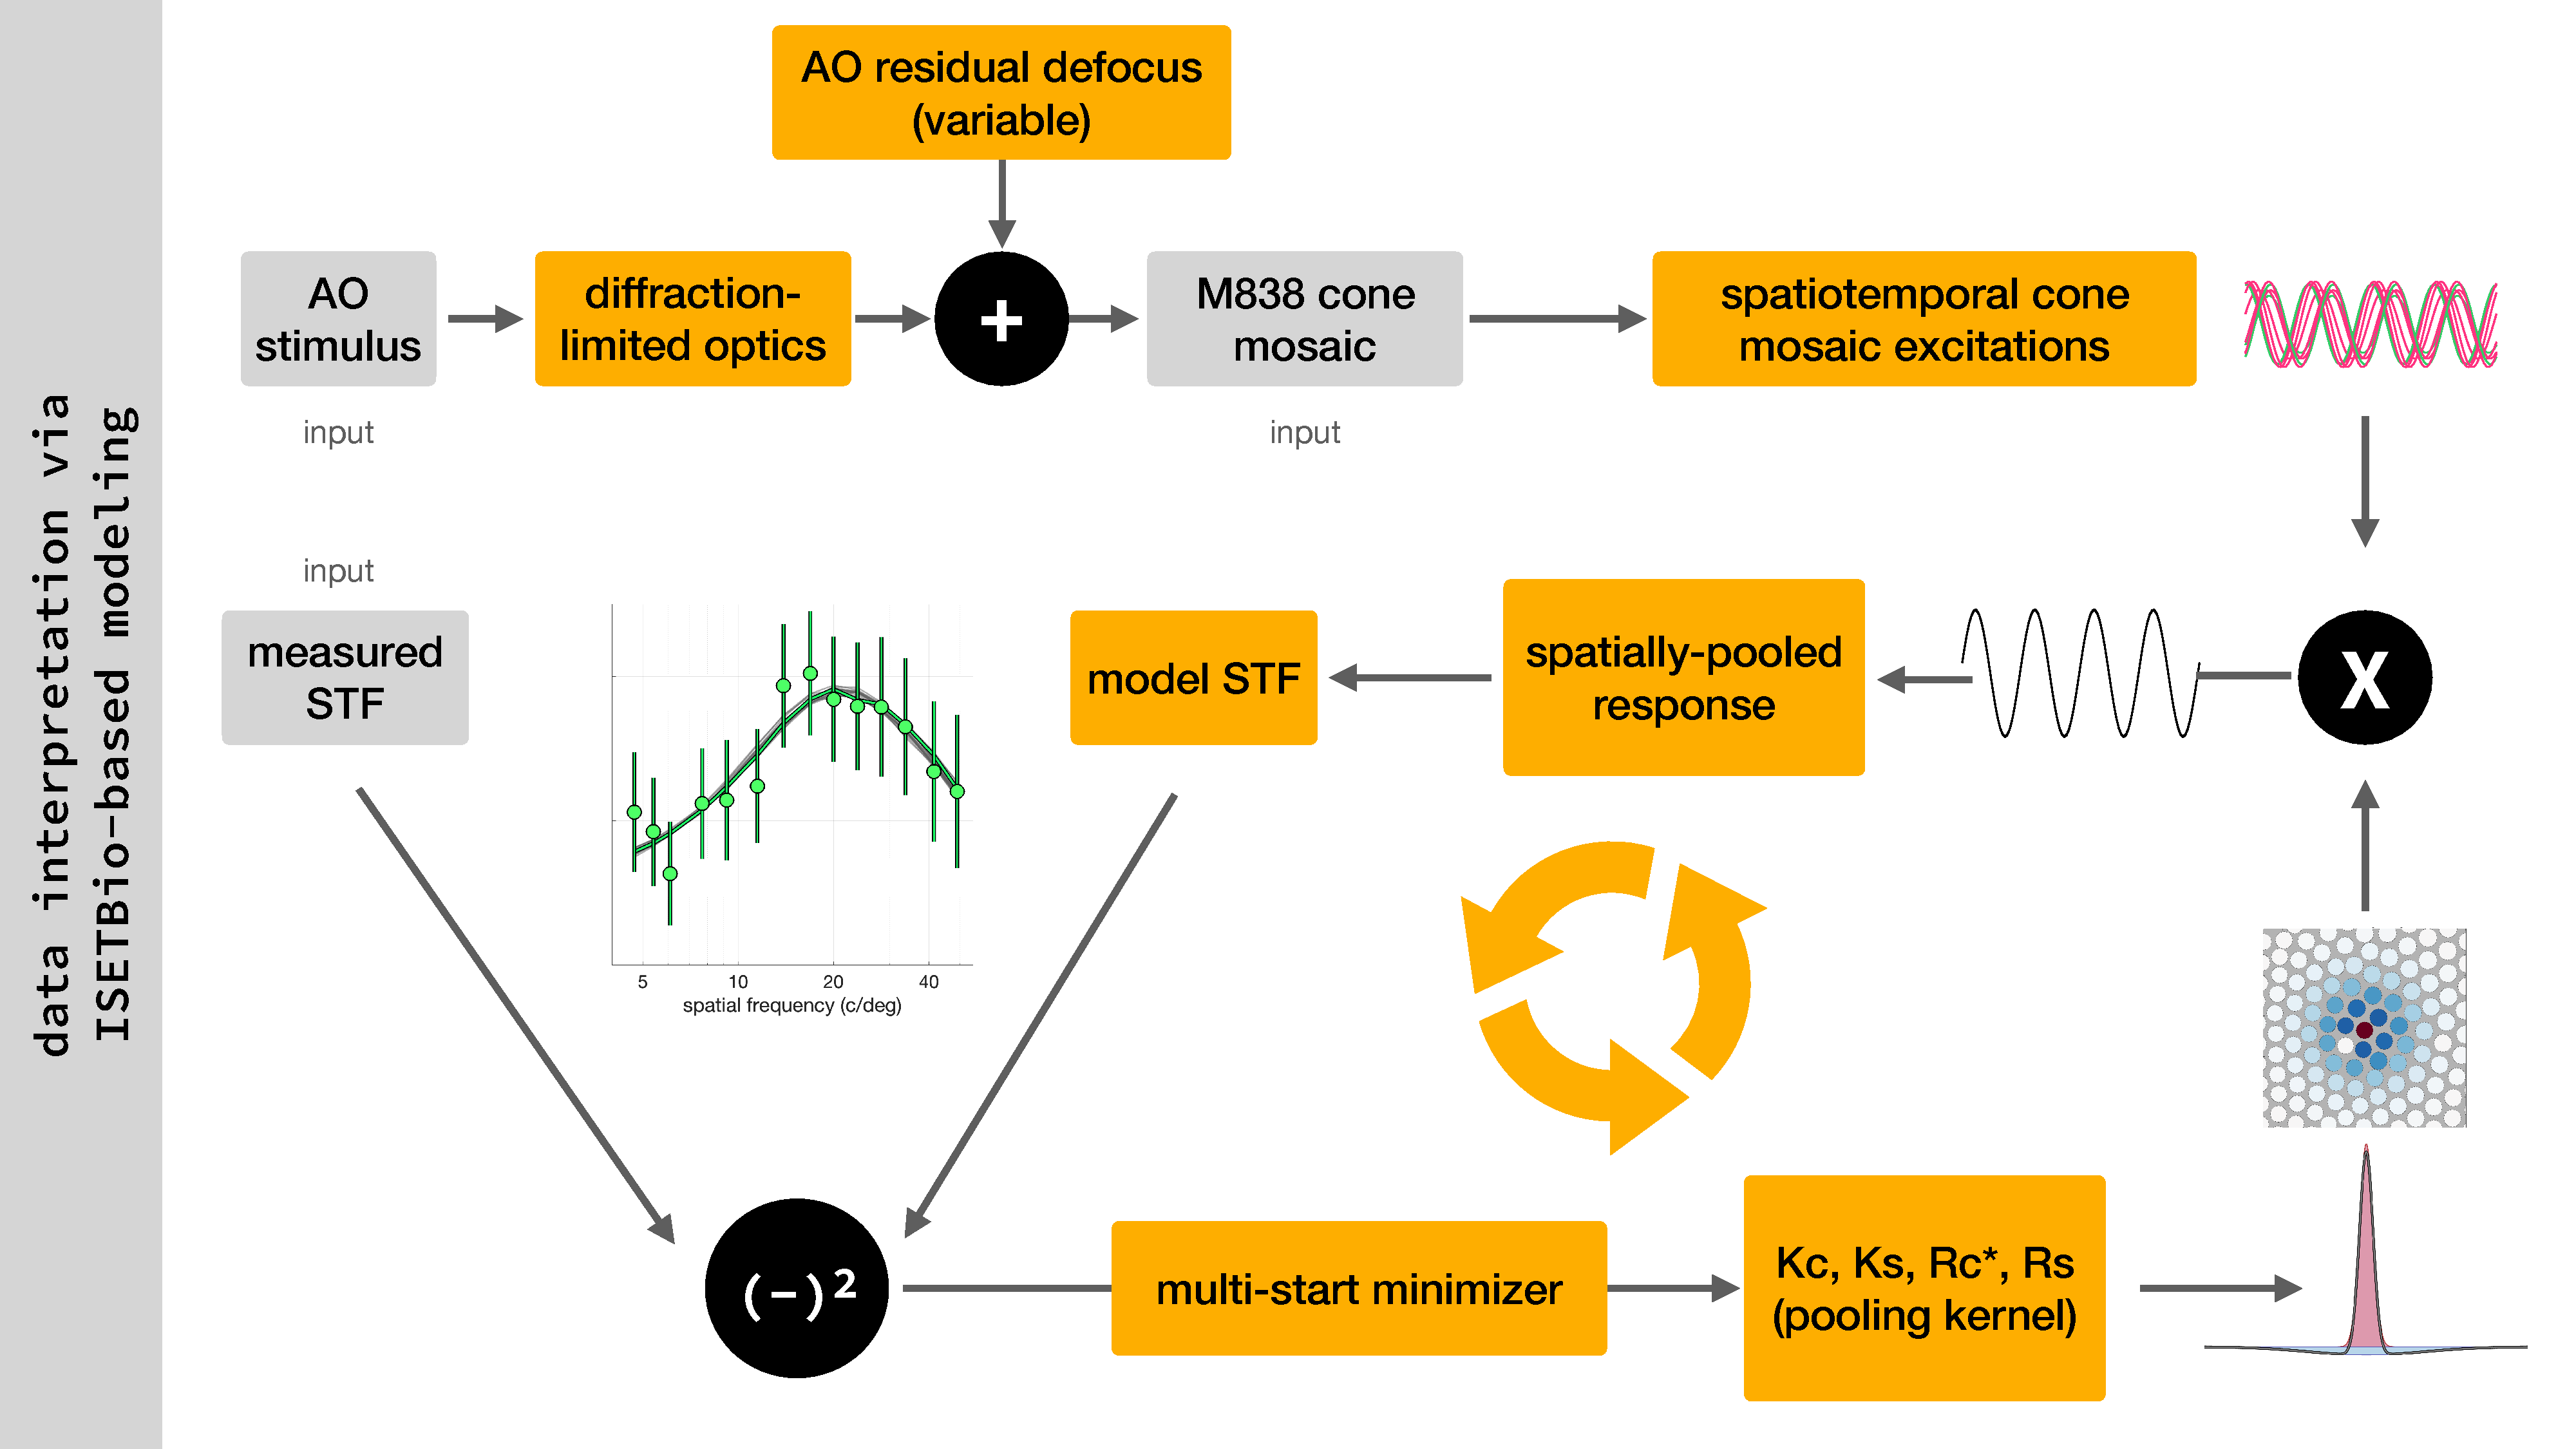
\includegraphics[width=7in]{Figures/ModelOverview.pdf} 
   \caption{Schematic overview of the ISETBio computational model.}
   \label{fig:ModelOverview}
\end{figure}


\begin{figure}[htbp] %  figure placement: here, top, bottom, or page
   \centering
   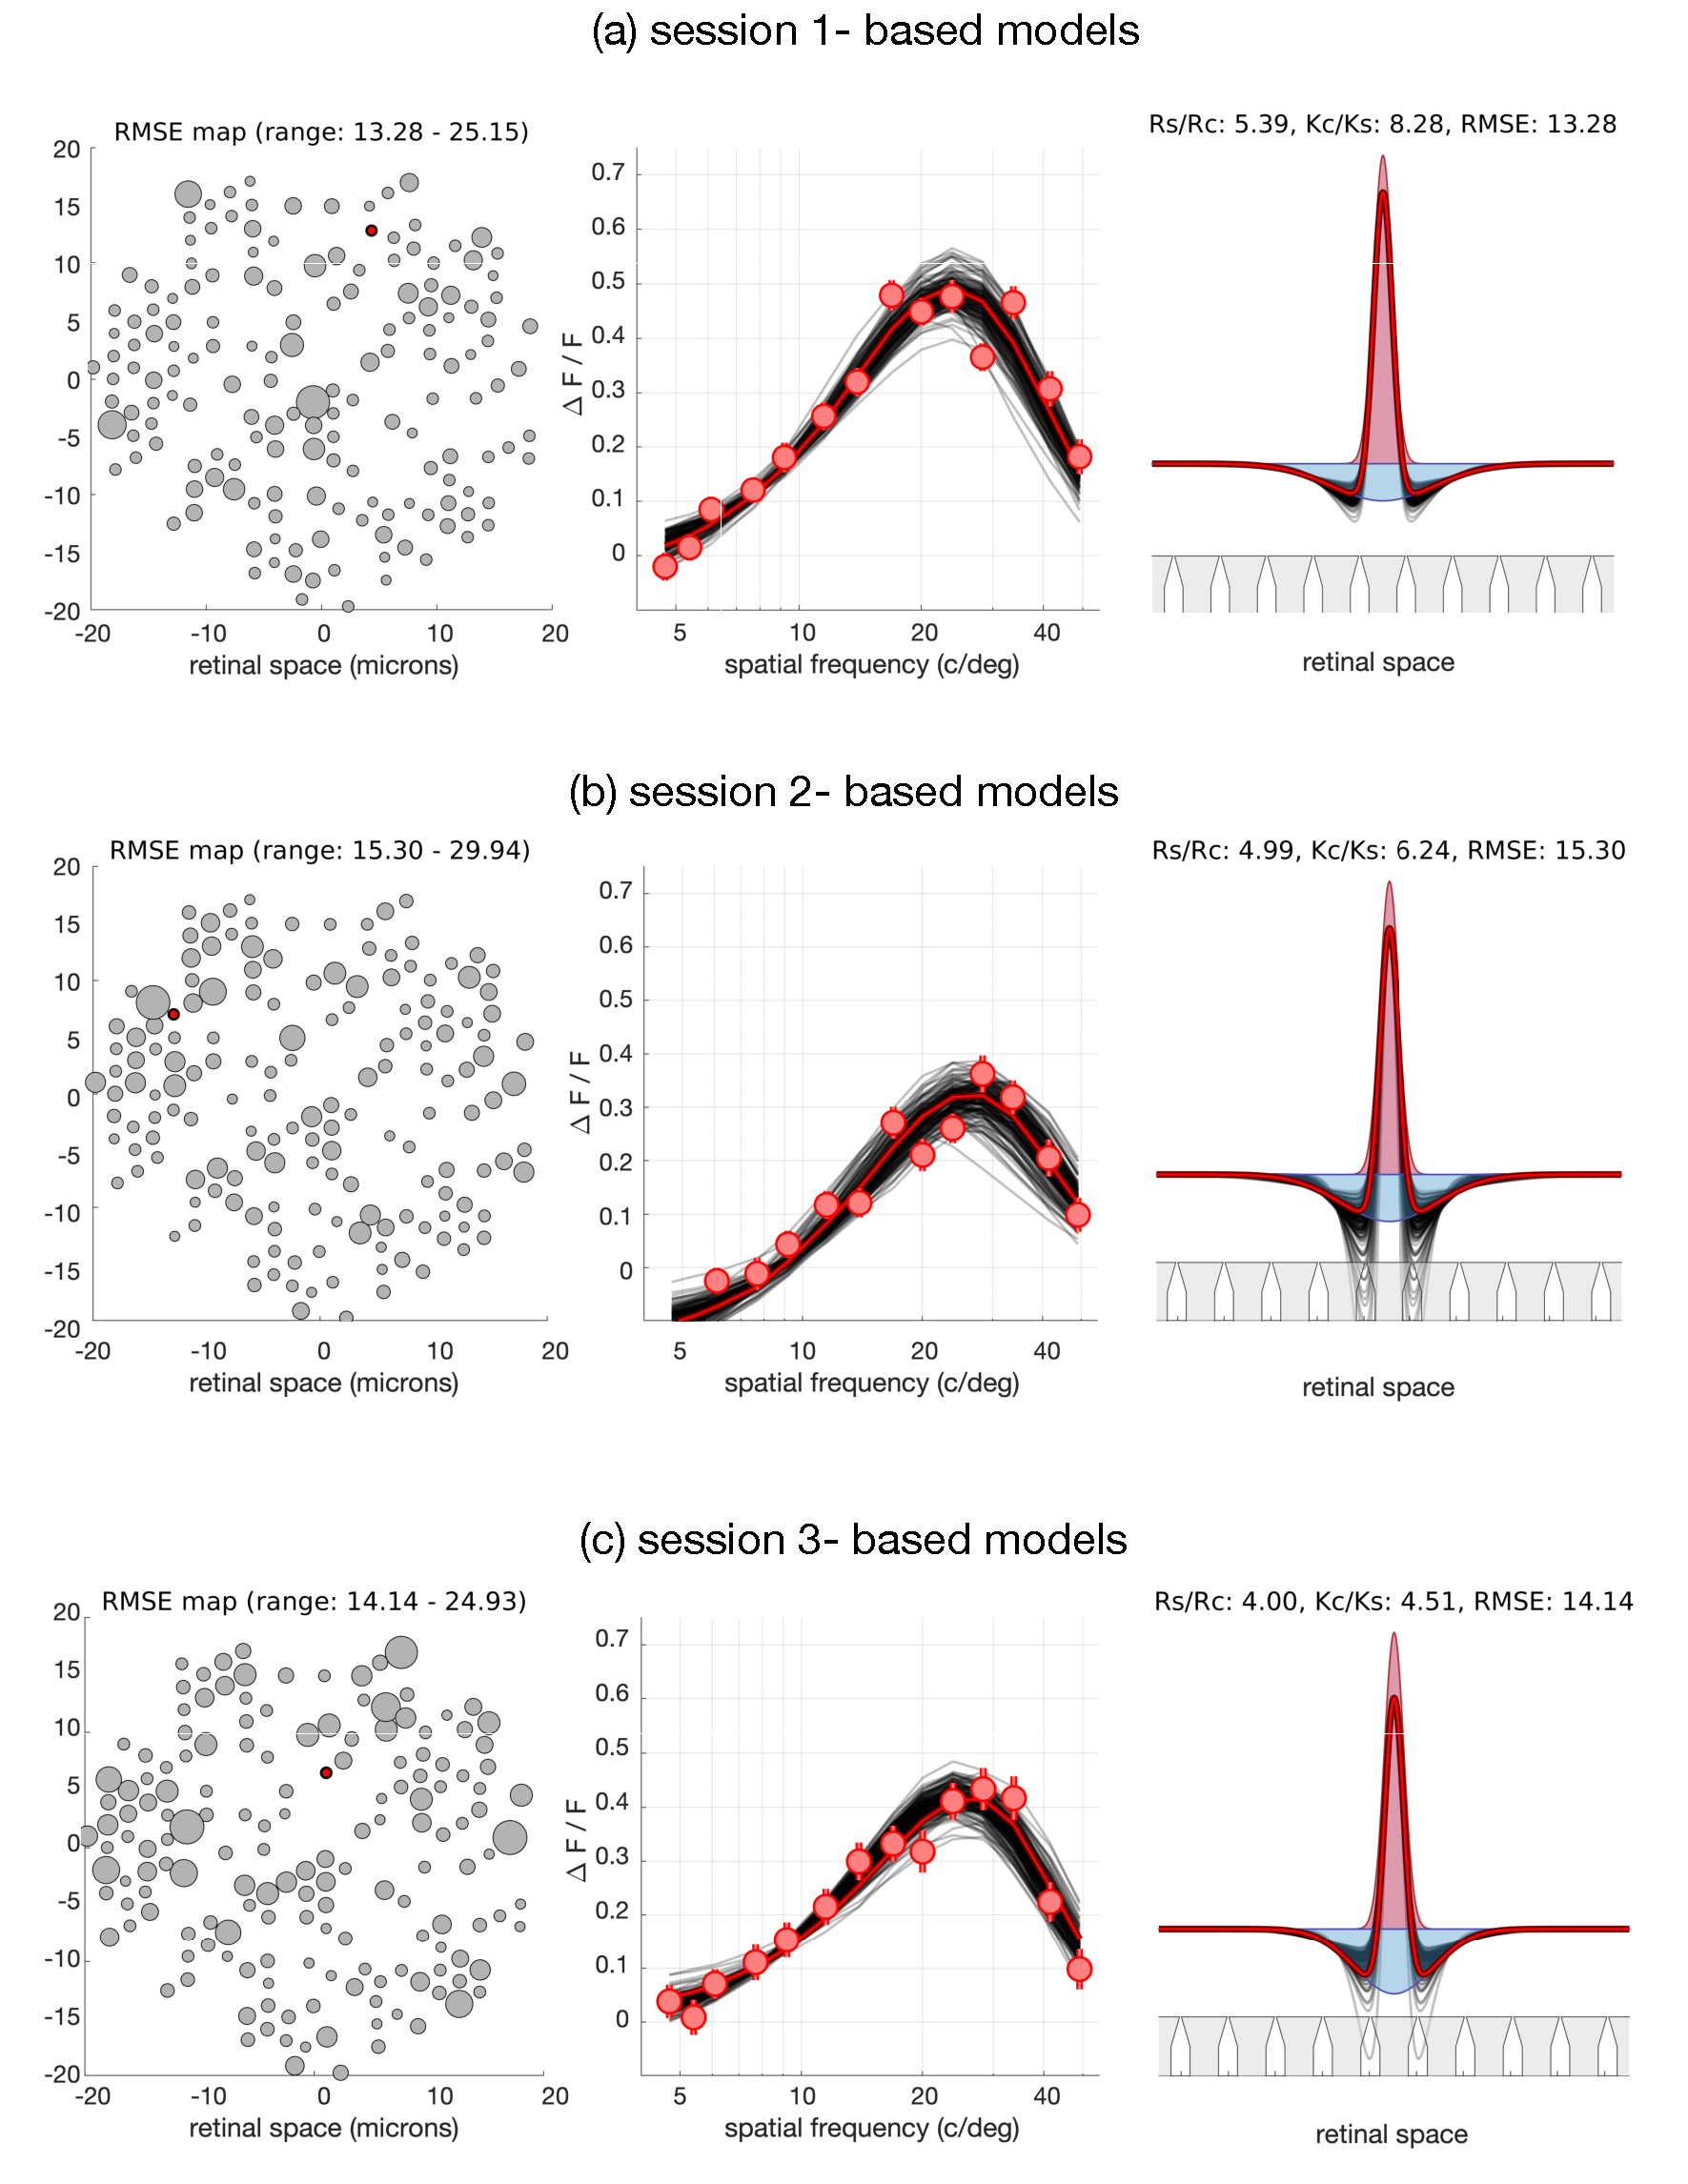
\includegraphics[width=6in]{Figures/CrossValidationMethod_TrainingModels.pdf} 
   \caption{Training RF models for an L-cone center RGC based on STF data recorded during the first (\textbf{A}), second (\textbf{B}) and third (\textbf{C}) recording session. \textbf{Left panels}: spatial map of RMSE between model STF and measured STF, as a function of center cone position in the examined model. There are a total of 161 models, each centered on one of 161 cones within the mosaic. Bubble size denotes magnitude of RMSE for each model. \textbf{Middle panels}: Fits of model STF (black lines) to the measured STF data (red disks) for all 161 examined models. The red line represents the best fit. \textbf{Right panels}: Black thin traces depict the RF profiles of the 161 examined models. The red thick line depicts the RF profile of the best fit model, whereas the pink and blue shaded areas depict the center and surround mechanism profiles of the best fit model. The apertures of cones are depicted schematically in gray.}
   \label{fig:CrossValidationApproach_TrainingModels}
\end{figure}

\begin{figure}[htbp] %  figure placement: here, top, bottom, or page
   \centering
   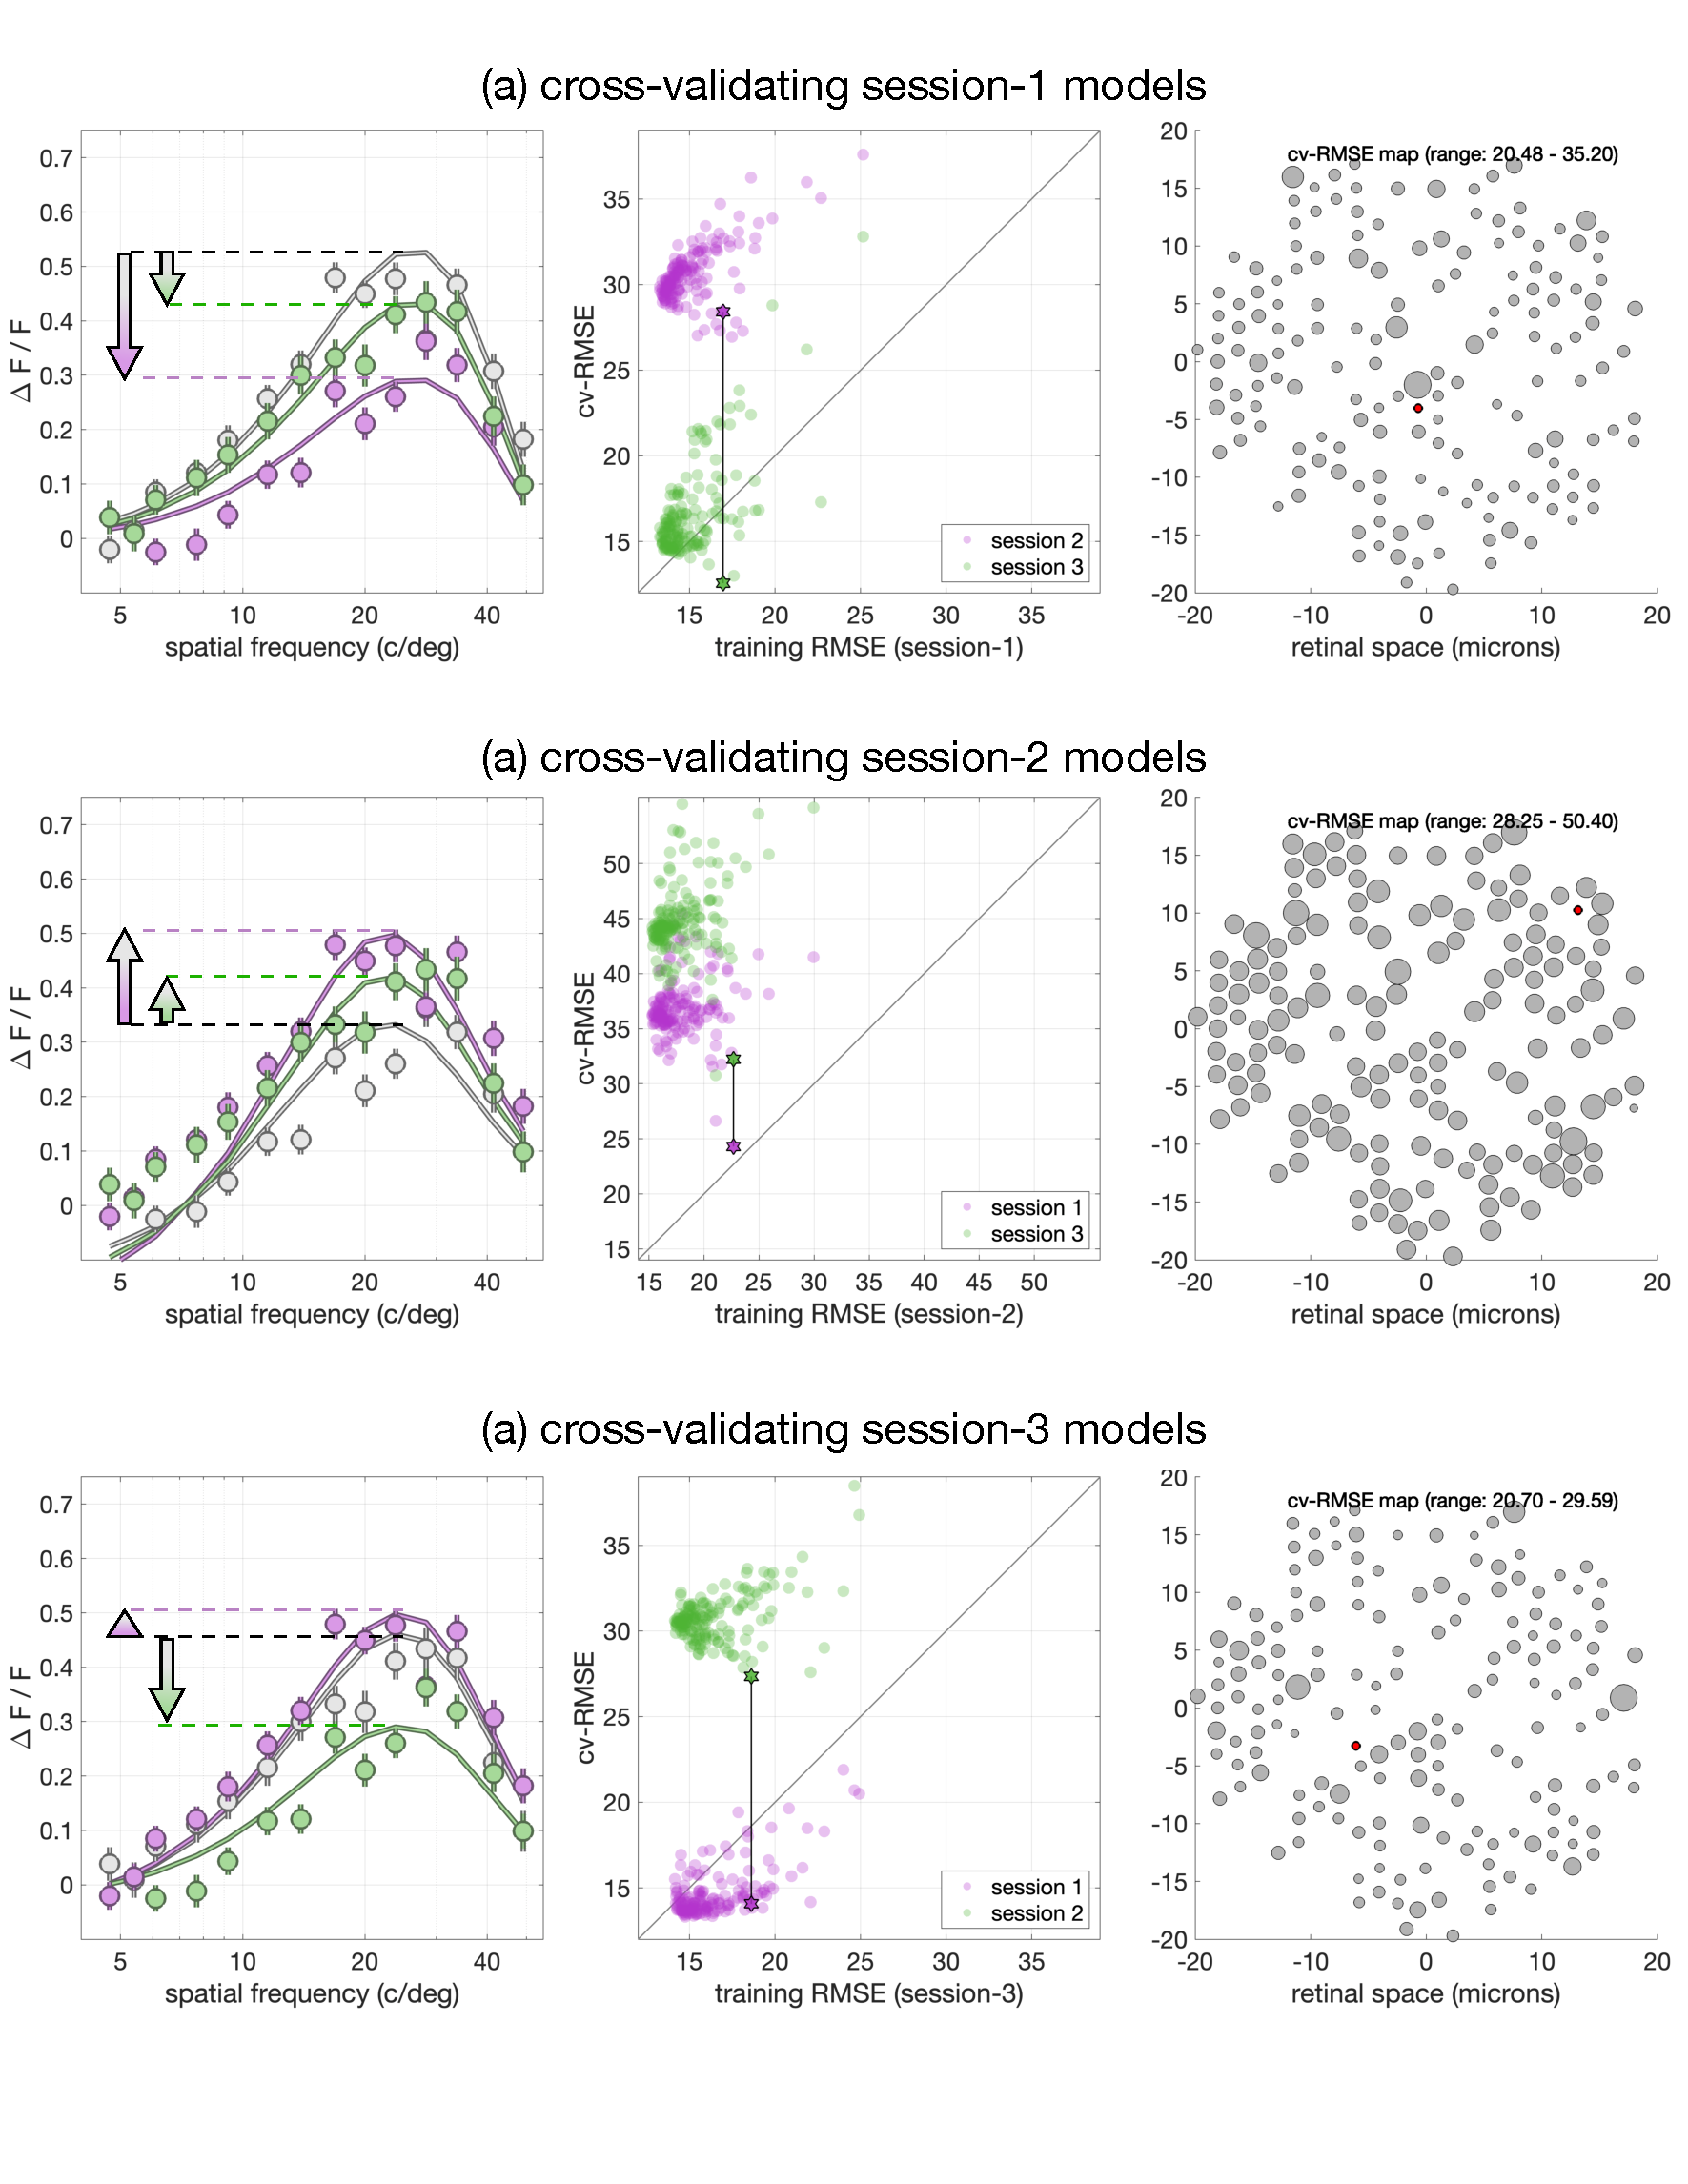
\includegraphics[width=6in]{Figures/CrossValidationMethod_CrossValidatingSession1Models.pdf} 
   \caption{Cross-validating RF models for the same L-cone center RGC cell. The model RF is trained on STF data recorded during the first recording session (\textbf{A}), the second session (\textbf{B}) and third session (\textbf{C}). \textbf{Left panels}: Gray lines depict the STF of the model RF trained in the current session that resulted in the minimum combined cross-validation error over the remaining 2 sessions, across all examined cone positions. Green and purple lines, depict the optimal cross-validated fits along with the scaling factor (arrows) that had to be applied to derive them from the STF of the model RF.  \textbf{Middle panels}: The cross-validated errors are plotted against the training errors for all examined cone positions. The connected stars indicate where the minimum combined cross-validated error occurred. \textbf{Right panels}: Spatial map of cross-validated errors, with bubble size indicated the error magnitude. The position of the cone at which this minimum occurred is denoted by the red circle.
    }
 \label{fig:CrossValidationApproach_CrossValidatingModels}
\end{figure}


\begin{figure}[htbp] %  figure placement: here, top, bottom, or page
   \centering
   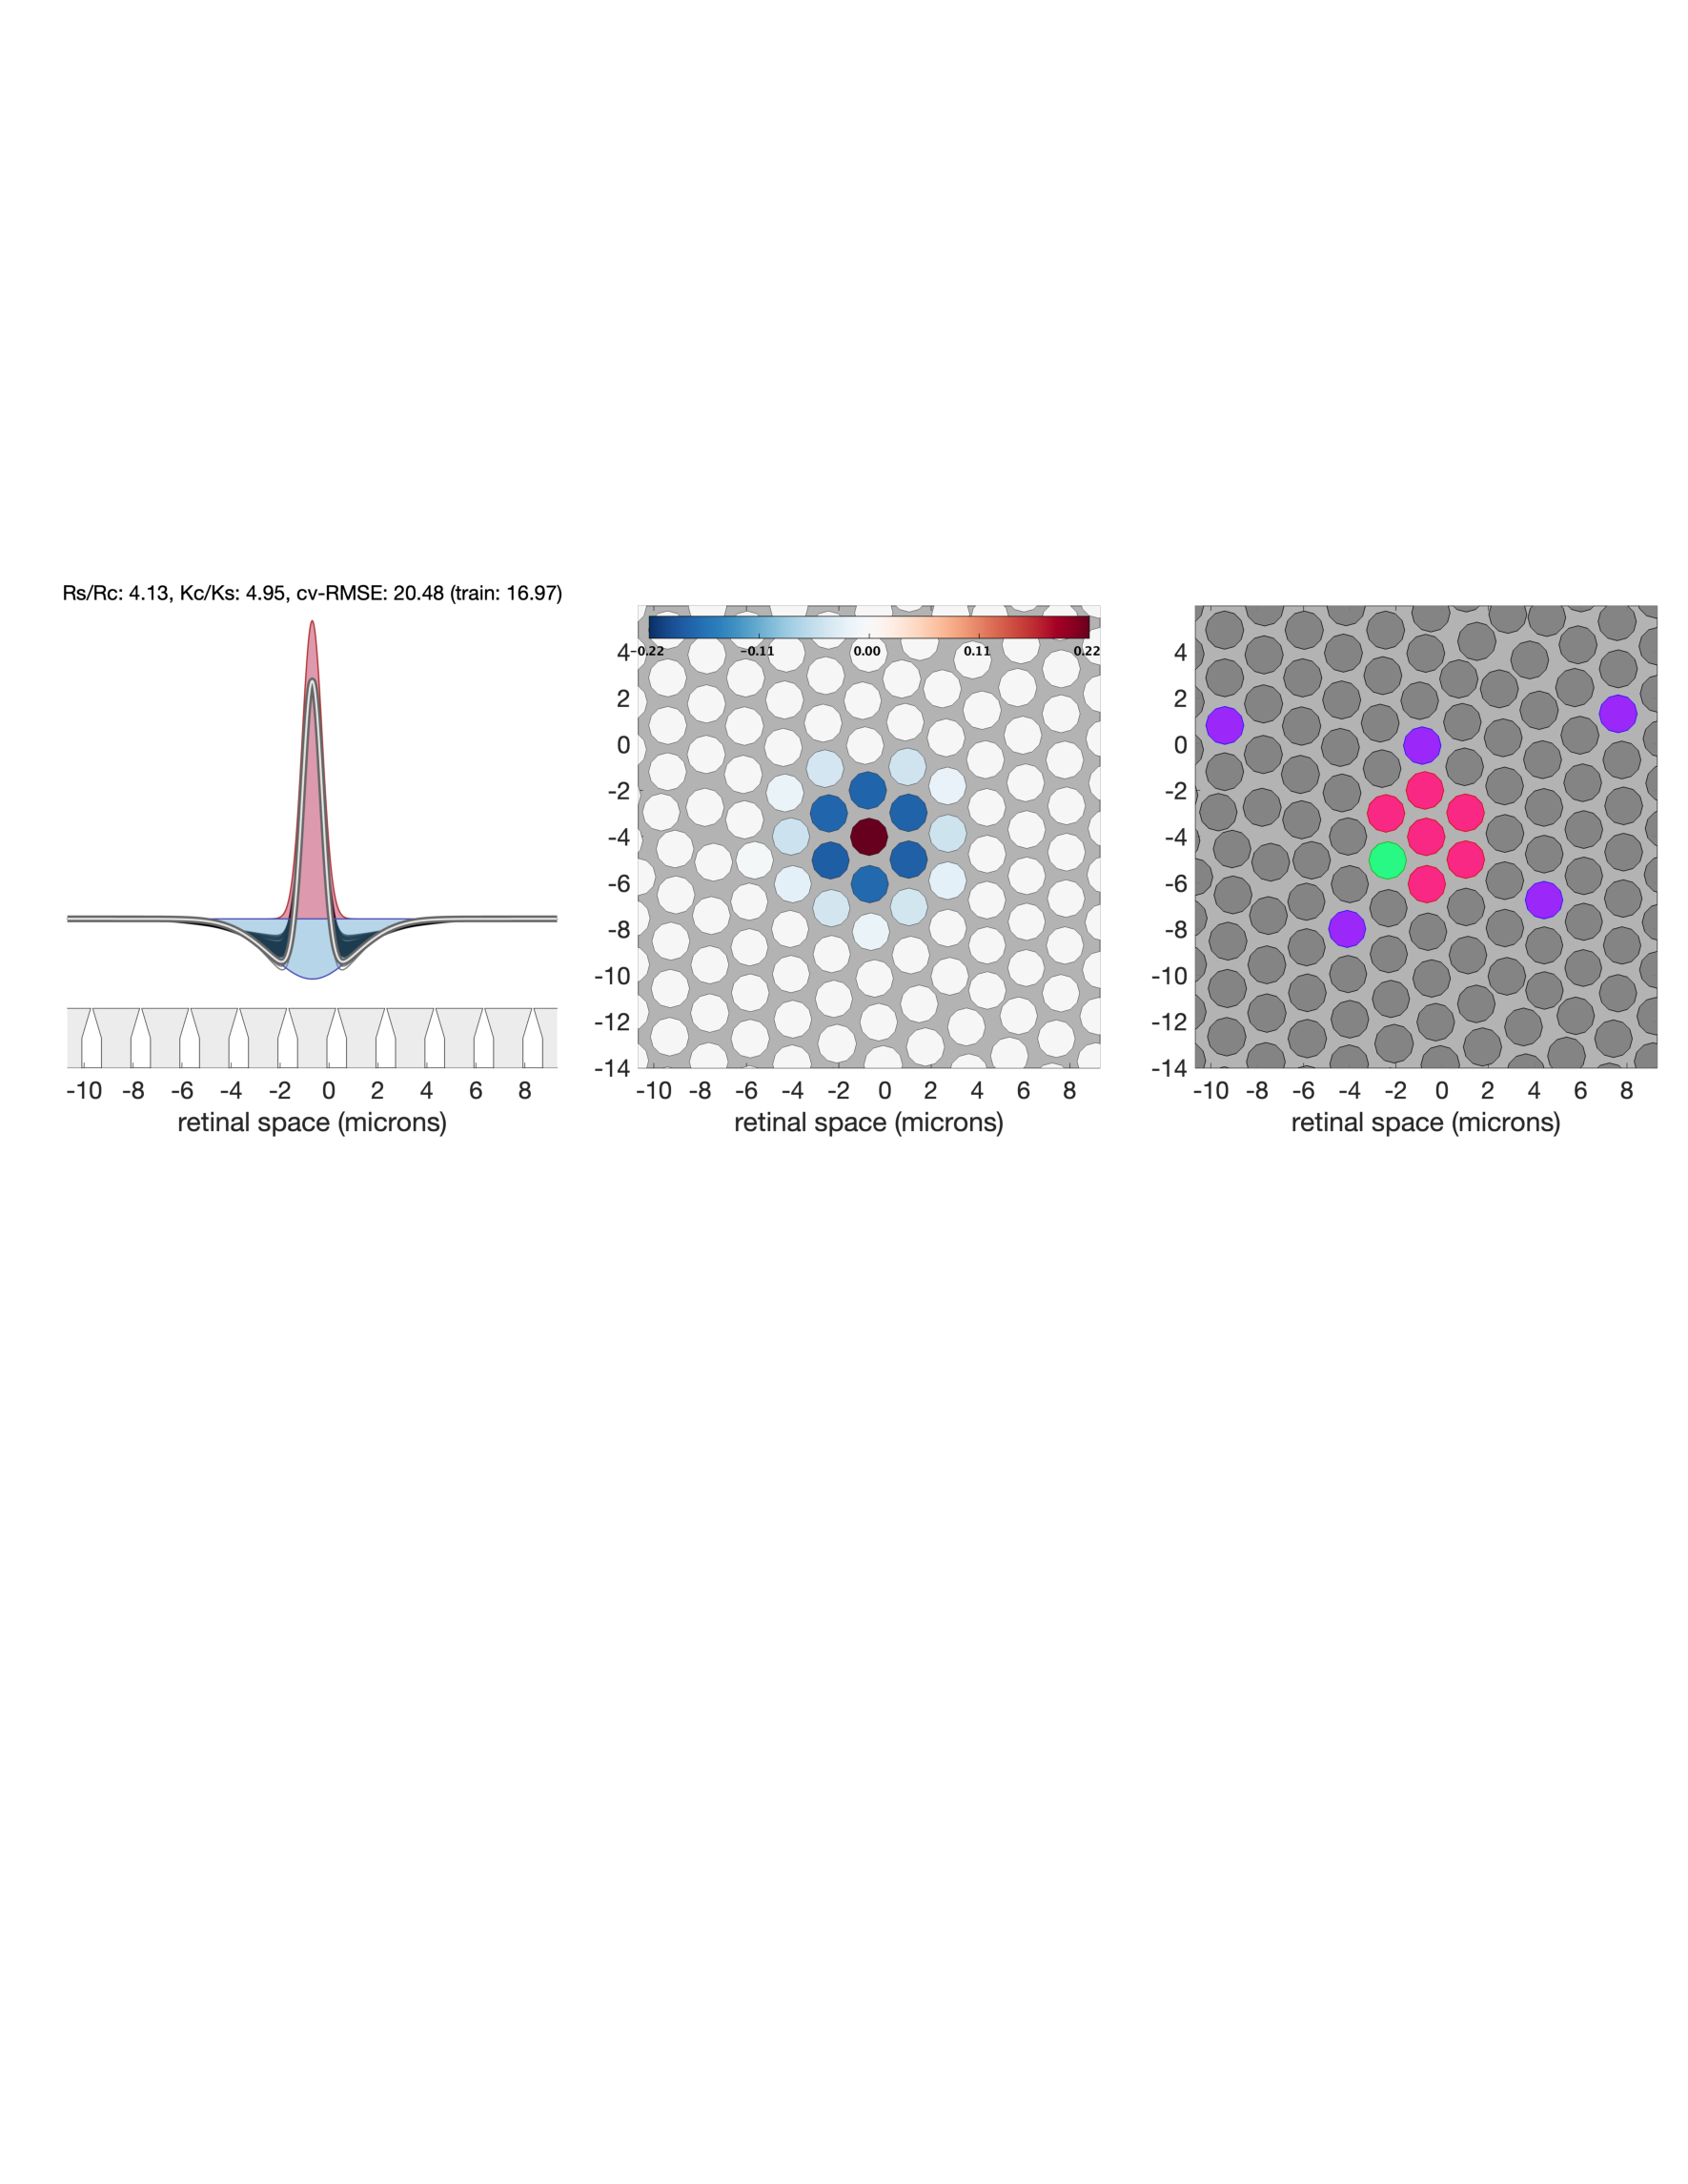
\includegraphics[width=6in]{Figures/CrossValidationMethod_BestCrossValidatedModel.pdf} 
   \caption{Best cross-validated RF model. \textbf{Left panel :} The RF profile of the best fit model, is depicted by the white thick line, whereas the pink and blue shaded areas depict the profiles of the center and surround mechanisms, respectively. Cone apertures are depicted schematically in gray below.  \textbf{Middle panel:} Weights of cones feeding into the RF center (red) and the RF surround (blue) mechanisms. \textbf{Right panel:} Labeling of L/M- (red/green) cones whose weights to the best cross-validated RF model are greater than 5\% of the center cone weight, or are S-cones (blue).
   }
 \label{fig:CrossValidationApproach_BestCrossValidatedModel}
\end{figure}

\newpage
\newpage





\end{document}  